\section{Soporte Vital Inmediato}
El Soporte Vital Inmediato (SVI) es un conjunto de medidas y técnicas médicas que se aplican a una persona que ha sufrido una emergencia médica grave para estabilizar sus signos vitales y prevenir el agravamiento de su estado de salud hasta que se pueda proporcionar un tratamiento especializado. El SVI incluye medidas como la reanimación cardiopulmonar, oxigenoterapia, la intubación traqueal, la administración de líquidos intravenosos y medicamentos, y la realización de procedimientos invasivos para controlar la hemorragia, estabilizar fracturas y lesiones, y asegurar la permeabilidad de las vías respiratorias.

El objetivo del SVI es mantener la función de los órganos vitales del cuerpo para evitar el daño irreversible y la muerte.

\subsection{Estaciones y cronograma}
Las estaciones y el cronograma se hacen de acuerdo a lo hecho en el curso de SVI de noviembre de 2022. 

% Please add the following required packages to your document preamble:
% \usepackage{multirow}
% \usepackage[table,xcdraw]{xcolor}
% If you use beamer only pass "xcolor=table" option, i.e. \documentclass[xcolor=table]{beamer}
\begin{table}[hptb]
    \centering
    \begin{tabular}{ccccc}
    \rowcolor[HTML]{333333} 
    {\color[HTML]{FFFFFF} Día} & {\color[HTML]{FFFFFF} Duración} & {\color[HTML]{FFFFFF} Grupo A} & {\color[HTML]{FFFFFF} Grupo B} & {\color[HTML]{FFFFFF} Grupo C} \\
     & 1 H & \multicolumn{3}{c}{Explicación Teórica} \\
     & \cellcolor[HTML]{D9D9D9}45 min & \multicolumn{3}{c}{\cellcolor[HTML]{D9D9D9}RCP básica} \\
     & 45 min & \multicolumn{3}{c}{Aproximación ABCDE} \\
     & \cellcolor[HTML]{D9D9D9}15/30 min & \multicolumn{3}{c}{\cellcolor[HTML]{D9D9D9}Descanso} \\
     & 45 min & Vía aérea & Acceso Vascular, fármacos & Monitorización y arritmias \\
     & \cellcolor[HTML]{D9D9D9}45 min & \cellcolor[HTML]{D9D9D9}Monitorización y arritmias & \cellcolor[HTML]{D9D9D9}Vía aérea & \cellcolor[HTML]{D9D9D9}Acceso Vascular,  fármacos \\
    \multirow{-7}{*}{Día I} & 45 min & Acceso Vascular, fármacos & Monitorización y arritmias & Vía aérea \\ \hline
    \rowcolor[HTML]{D9D9D9} 
    \cellcolor[HTML]{D9D9D9} & 1 H & \multicolumn{3}{c}{\cellcolor[HTML]{D9D9D9}Escenarios de SVI y desfibrilación} \\
    \cellcolor[HTML]{D9D9D9} & 30 min & \multicolumn{3}{c}{Demostración SVI integrado} \\
    \rowcolor[HTML]{D9D9D9} 
    \cellcolor[HTML]{D9D9D9} & 1 H & \multicolumn{3}{c}{\cellcolor[HTML]{D9D9D9}Escenario Integrado SVI} \\
    \cellcolor[HTML]{D9D9D9} & 20 min & \multicolumn{3}{c}{Descanso} \\
    \rowcolor[HTML]{D9D9D9} 
    \multirow{-5}{*}{\cellcolor[HTML]{D9D9D9}Día II} & $\mathbb{N}$ min & \multicolumn{3}{c}{\cellcolor[HTML]{D9D9D9}Evaluación} \\ \hline
    \end{tabular}
    \caption{Estaciones propuestas para SVA junto con su duración}
    \label{tab:Brusilov:SVI:Estaciones}
\end{table}

% Please add the following required packages to your document preamble:
% \usepackage[table,xcdraw]{xcolor}
% If you use beamer only pass "xcolor=table" option, i.e. \documentclass[xcolor=table]{beamer}
\begin{table}[hptb]
    \centering
    \begin{tabular}{N{0.24\textwidth}N{0.15\textwidth}M{0.54\textwidth}}
        \rowcolor[HTML]{333333} 
        {\color[HTML]{FFFFFF} Estación} & {\color[HTML]{FFFFFF} Sala propuesta} & {\color[HTML]{FFFFFF} Equipamiento} \\
        Explicación teórica & Aula 2 & Ordenador, Pantalla, Sillas \\
        \rowcolor[HTML]{D9D9D9} 
        RCP Básica & Simulación 1, Simulación 2, Simulación 3 & Busto RCP, DEA Laerdal \\
        Aproximación ABCDE & Simulación 1, Simulación 2, Simulación 3 & Sillas \\
        \rowcolor[HTML]{D9D9D9} 
        Vía Aérea, Oxigenoterapia y Ventilación & Simulación 1 & Gafas Nasales, Mascarillas faciales (con reservorio, efecto Venturi), Cánula de Guedel, Mascarilla laríngea (clásica, iGel), Fastrach (Fastrach, tubo de Brian, intercambiador), Tubo endotraqueal, Laringoscopio, Froba, Fiador, Kit cricotirotomía, Airtraq, Sonda Yankauer, Tubuladuras para respirador, Ambú, Busto para intubación \\
        Acceso Vascular, líquidos y fármacos & Simulación 2 & Abbocat de distintos tamaños, pistola intraósea, aguja para intraósea, muslo de pollo y huevos, brazo para venopunción \\
        \rowcolor[HTML]{D9D9D9} 
        Monitorización y Arritmias & Simulación 3 & Desfibrilador, maniquí simulador arritmias, DEA \\
        Escenarios SVI y desfibrilación & Simulación 1, Simulación 2, Simulación 3 & Sillas \\
        \rowcolor[HTML]{D9D9D9} 
        Escenarios Integrados SVI/Demostración SVI & Simulación 3 y Aula 2 & Abbocat de distintos tamaños, ampollas medicación Mock, Sueros y sistemas de suero, Gafas Nasales, Mascarillas faciales (con reservorio, efecto Venturi), Cánula de Guedel, Mascarilla laríngea (clásica, iGel), Fastrach (Fastrach, tubo de Brian, intercambiador), Tubo endotraqueal, Laringoscopio, Froba, Fiador, Tubuladuras para respirador, Aula 2 (Sistema Intuity, Ordenador, Pantalla) \\ \hline
    \end{tabular}
    \caption{Salas y material propuesto para cada estación descrita}
    \label{tab:Brusilov:SVI:SalasEstaciones}
\end{table}

Así, el listado de materiales queda (según lo pedido en la información dada):
\begin{itemize}[topsep=0pt, partopsep=0pt,itemsep=0pt,parsep=0pt]
    \item \textbf{Medicación y Material de vía venosa}:
    \begin{itemize}[topsep=0pt, partopsep=0pt,itemsep=0pt,parsep=0pt]
        \item 30 Apósitos.
        \item Catéter Abbocat (30 del 24G, 30 del 22G, 30 del 20G, 2 del 18G, 2 del 16G, 2 del 14G).
        \item 2 Compresor.
        \item Bolsa de Sangre y de Plasma para transfusiones.
        \item Material de intraósea (pistola de intraósea, agujas para intraósea).
        \item Ampollas de Medicación Mock (reetiquetar suero fisiológico de uso tópico):
        \vspace{-12.5pt}
        \begin{multicols}{2}
            \begin{itemize}[topsep=0pt, partopsep=0pt,itemsep=0pt,parsep=0pt]
                \item Ácido tranexámico 500 mg (100 mg/mL).
                \item Adrenalina 1 mg/mL.
                \item Alteplasa 100 mg (20 mg/mL).
                \item Amiodarona 150 mg (50 mg/mL).
                \item Atropina 1 mg/mL.
                \item Bicarbonato sódico 1 M (8.5 mg/mL).
                \item Bicarbonato sódico 1.6 M (14 mg/mL).
                \item Cloruro Sódico 20 \% (200 mg/mL).
                \item Cloruro Cálcico 100 mg (100 mg/mL).
                \item Cloruro Potásico 20 mEq (2mEq/mL).
                \item Digoxina 0.5 mg (0.25 mg/mL).
                \item Dopamina 200 mg (40 mg/mL).
                \item Etomidato 20 mg (2 mg/mL).
                \item Fentalino 0.5 mg (0,15 mg/mL).
                \item Fibrinógeno 1 g (20 mg/mL).
                \item Hidrocortisona 100 mg (20 mg/mL).
                \item Hidroxicobalamina 100 mg (5000 $\mu$g/mL).
                \item Labetalol 100 mg (5 mg/mL).
                \item Lidocaína 2 \% 200 mg (20 mg/mL).
                \item Matamizol magnésico 2g (0.04 mg/mL).
                \item Midozalam 15 mg (5mg/mL).
                \item Morfina 10 mg/mL
                \item Nitroglicerina 50 mg (5 mg/mL).
                \item Noradrenalina 10 mg (2 mg/mL).
                \item Propofol 200 mg (10 mg/mL).
                \item Rocuronio 50 mg (10 mg/mL)
                \item Sulfato magnésico 1,5 mg (150 mg/mL).
                \item Urapidilo 50 mg (5 mg/mL).
            \end{itemize}
        \end{multicols}
    \end{itemize}
    \item \textbf{Material de vía aérea}:
    \begin{itemize}[topsep=0pt, partopsep=0pt,itemsep=0pt,parsep=0pt]
        \item Busto de intubación Laerdal.
        \item 2 Gafas Nasales.
        \item 4 Mascarillas faciales (2 efecto Venturi, 2 con reservorio).
        \item Canulas de Guedel (2 de cada calibre).
        \item 2 Mascarillas laríngeas clásicas Calibre 3.
        \item Mascarillas laríngeas iGel (2 de cada calibre).
        \item 2 Mascarillas Fastrach (calibre 3), junto con tubo de Brian e intercambiador.
        \item Tubo orotraqueal (2 de cada calibre: 6, 6.5, 7, 7.5, 8).
        \item 2 Laringoscopios.
        \item 2 Airtraq
        \item 2 Botes de lubricante para intubación.
        \item 2 Sonda Yankauer, junto con sistema de vacio.
        \item 2 Pinzas de Magill.
        \item Kit de cricotirotomía.
        \item 2 Tubuladuras de respirador.
    \end{itemize}
    \item \textbf{Otros}:
    \begin{itemize}[topsep=0pt, partopsep=0pt,itemsep=0pt,parsep=0pt]
        \item Drenaje con sangre.
        \item Pleurevac.
        \item Sábana Pélvica.
        \item Collarín.
        \item Tubo de tórax.
        \item Vendas.
        \item Catéter Central de Inserción Periférica (PICC).
    \end{itemize}
\end{itemize}

\clearpage

\section{Casos Codificados}
\subsection{Caso A - Asistolia por Shock hipovolémico}
\paragraph{Escenario} UCI
\vspace{-12.5pt}
\paragraph{Paciente} Varón de 60 años, hipertenso y obeso. Intervenido resección sigma hace 12 horas. El paciente presenta una hipotensión brusca (70/40 mmHg), taquicardia sinusal (110 lpm), sudoración y malestar general tras administrar un nolotil intravenoso. El paciente lleva un drenaje abdominal con débito hemático.
\vspace{-12.5pt}
\paragraph{Caso} Enfermería avisa al personal médico de guardia. Paciente relata que le han operado, tras 100 segundos, pierde conocimiento (deja de hablar) y deja de notarse el pulso. Desarrolla una Actividad Eléctrica Sin Pulso. Se espera que el alumnado realice el protocolo de RCP no desfibrilable:
\begin{enumerate}[topsep=0pt, partopsep=0pt,itemsep=0pt,parsep=0pt]
    \item Colocación de tablero de RCP.
    \item Inicio de compresiones y asistencia de vía aérea con Ambú (30:2).
    \item Canalización de vía venosa, junto con administración de medicación (adrenalina cada 3 minutos).
    \item Si el alumnado no progresa (sólo hace compresiones), recordar las posibles causas de parada (<<4H y 4T>>).
\end{enumerate}
\vspace{-12.5pt}
\paragraph{Pruebas complementarias}
\begin{itemize}[topsep=0pt, partopsep=0pt,itemsep=0pt,parsep=0pt]
    \item\textbf{Gasometría de ingreso}: pH 7,40; pCO$_2$ 45; pO$_2$ 20; EB -3; lact 8; Hb 10; HCO$_3^-$ 25.
    \item \textbf{Gasometría antes de la parada}: pH 7,10; pCO$_2$ 50; pO$_2$ 20; EB -15; lact 8; Hb 7; HCO$_3^-$ 16.
    \item \textbf{Gasometría en parada}: pH 7,00; pCO$_2$ 50; pO$_2$ 20; EB -20; lact 8; Hb 5; HCO$_3^-$ 12.
    \item \textbf{Electrocardiograma}: \href{https://drive.google.com/file/d/1GqvXc-N3dV9uCyPzkvCrG4abnPIkZzwb/view?usp=share\_link}{Enlace Drive ECG}
    \item \textbf{Placa rayos X torácica}: \href{https://drive.google.com/file/d/13VFzIBswwJGnbaB4wLQZWEIJGqibEyjh/view?usp=share\_link}{Enlace Drive RX tórax}
\end{itemize}

\begin{figure}[hptb]
    \centering
    \begin{subfigure}{.5\textwidth}
      \centering
      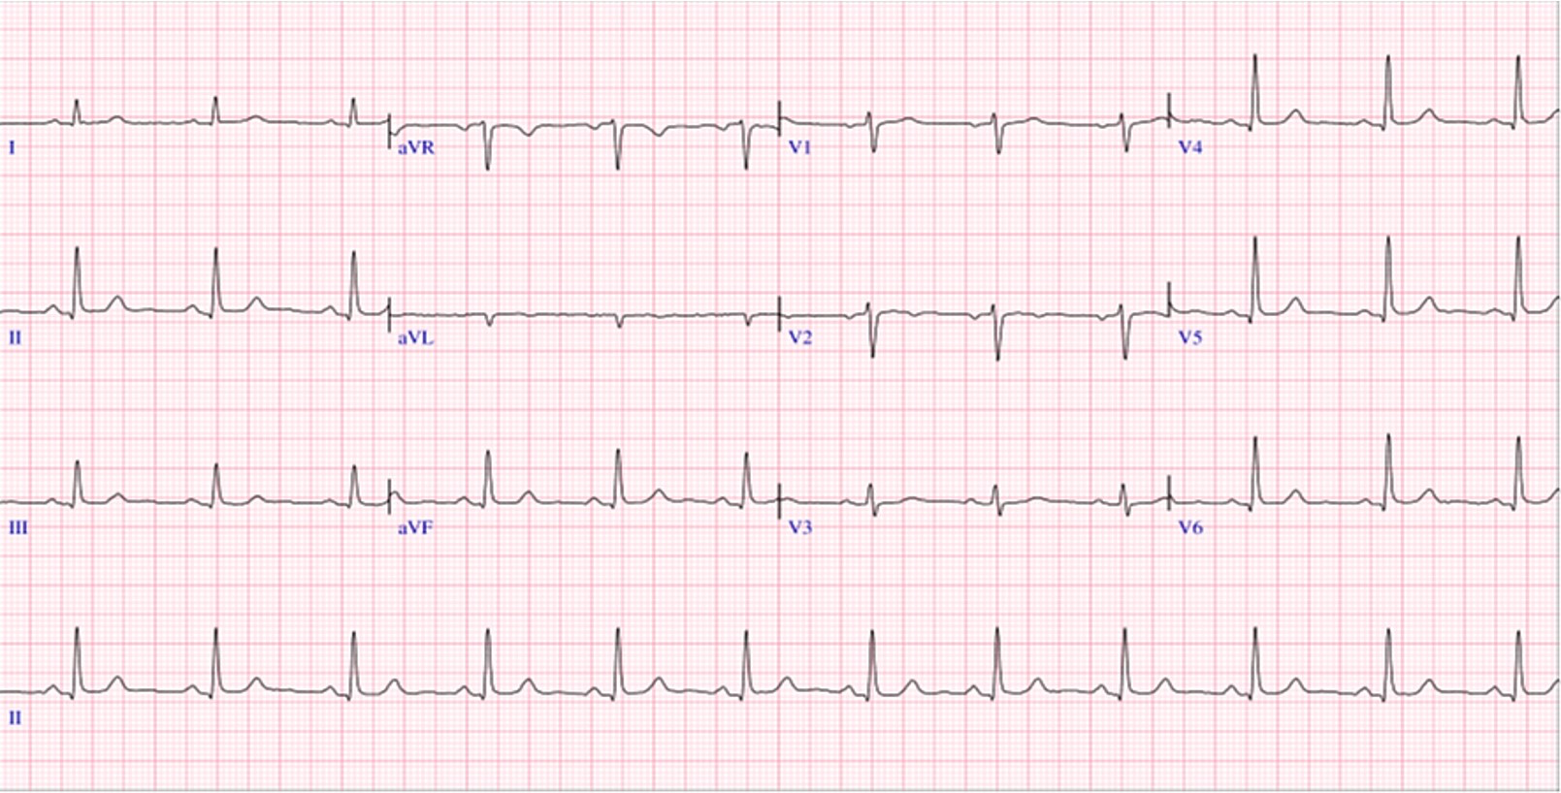
\includegraphics[width=0.5\textwidth]{./imagenes/UCIDoc-SVICasoAECG.png}
      \caption{\label{fig:Brusilov:SVI:CasoAECG}Electrocardiograma complementario.}
    \end{subfigure}%
    \begin{subfigure}{.5\textwidth}
      \centering
      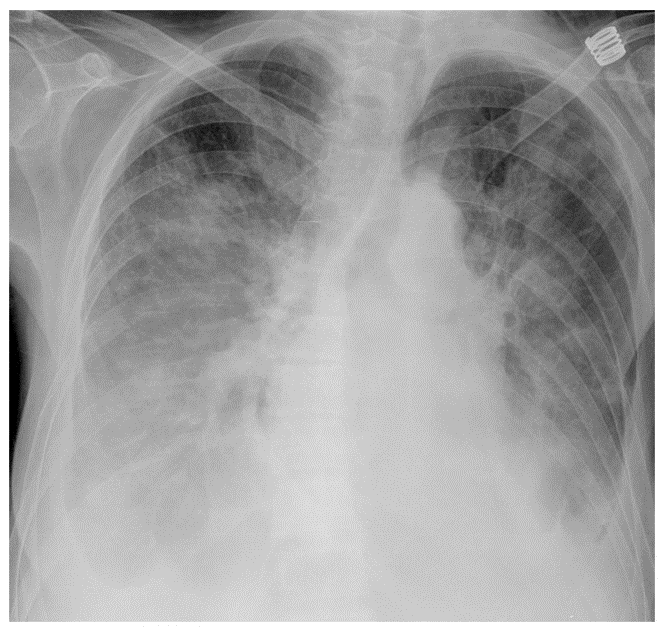
\includegraphics[width=0.3\textwidth]{./imagenes/UCIDoc-SVICasoARXTorax.png}
      \caption{\label{fig:Brusilov:SVI:CasoARXTorax}Placa de rayos X del tórax complementaria.}
    \end{subfigure}
    \caption{\label{fig:Brusilov:SVI:PruebasCasoA}Pruebas complementarias del Caso A.}
\end{figure}

\begin{figure}[hptb]
    \centering
	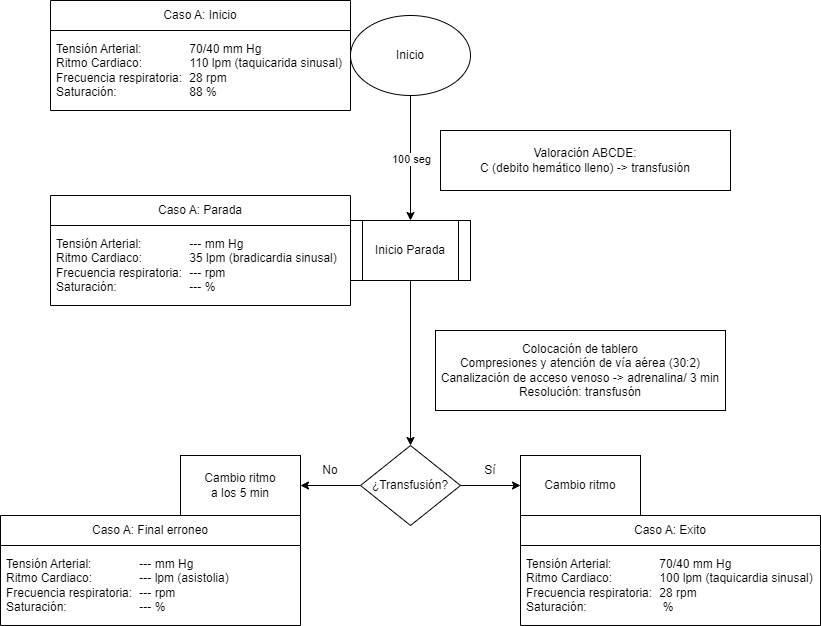
\includegraphics[width=0.766\linewidth]{./imagenes/ACV-AdSC-CasosUCI_CasoA.png}
	\caption{\label{fig:Brusilov:SVI:CasoA}Flujograma y resolución del Caso A.}
\end{figure}
\clearpage

\subsection{Caso B - Taquicardia Ventricular con Pulso}
\paragraph{Escenario} Urgencias
\vspace{-12.5pt}
\paragraph{Paciente} Mujer de 65 años acude a urgencias por unas palpitaciones, con un historial de CoVID hace 2 años y crisis de ansiedad de repetición. Ante la exploración, se encuentra fría, sudorosa, quejosa y con malestar general, taquicardia ventricular (180 lpm), hipotensión (85/40 mmHg), taquiapneica (30 rpm) y saturación de O$_2$ al 92\%.
\vspace{-12.5pt}
\paragraph{Caso} Se avisa al personal médico de guardia. El alumnado debe pedir un electrocardiograma y diagnosticar una taquicardia ventricular con pulso, cardiovertible. En el momento de cardiovertir (criterio opcional, conocer y/o recordar al alumnado la secuencia de analgosedación), existen dos caminos:
    \begin{itemize}[topsep=0pt, partopsep=0pt,itemsep=0pt,parsep=0pt]
        \item \textbf{Desfibrilación no sincronizada}: la paciente entra en fibrilación ventricular (FV).
        \item \textbf{Desfibrilación sincronizada}: la paciente se recupera durante un minuto y tras ello, entrar en FV.
    \end{itemize}
Se espera que el alumnado realice el protocolo de RCP desfibrilable:
\begin{enumerate}[topsep=0pt, partopsep=0pt,itemsep=0pt,parsep=0pt]
    \item Colocación de tablero de RCP.
    \item Inicio de compresiones y asistencia de vía aérea con Ambú (30:2).
    \item Desfibrilación precoz y administración cada dos min. Sale a la segunda desfibrilación.
    \item Canalización de vía venosa, junto con administración de medicación (adrenalina cada 3 minutos).
\end{enumerate}
\vspace{-12.5pt}
\paragraph{Pruebas complementarias}
\begin{itemize}[topsep=0pt, partopsep=0pt,itemsep=0pt,parsep=0pt]
    \item \textbf{Gasometría antes de la parada}: pH 7,30; pCO$_2$ 40; pO$_2$ 20; EB -8; lact 4; Hb 14; HCO$_3^-$ 19; K$^+$ 5.6.
    \item \textbf{Gasometría en parada}: pH 7,20; pCO$_2$ 40; pO$_2$ 20; EB -15; lact 8; Hb 14; HCO$_3^-$ 19; K$^+$ 6.
    \item \textbf{Electrocardiograma previo}: \href{https://drive.google.com/file/d/1GBe9Wofw9bwhYcRkuK_dNy-t5fBXRC2E/view?usp=share\_link}{Enlace Drive ECG}
    \item \textbf{Placa rayos X torácica}: \href{https://drive.google.com/file/d/13VFzIBswwJGnbaB4wLQZWEIJGqibEyjh/view?usp=share\_link}{Enlace Drive RX tórax}
\end{itemize}
\begin{figure}[hptb]
    \centering
    \begin{subfigure}{.5\textwidth}
      \centering
      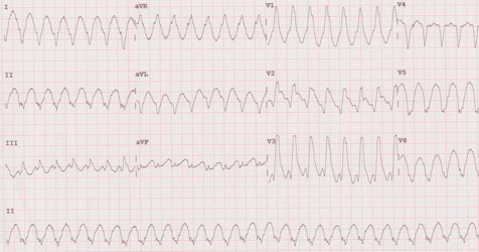
\includegraphics[width=0.5\textwidth]{./imagenes/UCIDoc-SVICasoBECG.png}
      \caption{\label{fig:Brusilov:SVI:CasoBECG}Electrocardiograma complementario.}
    \end{subfigure}%
    \begin{subfigure}{.5\textwidth}
      \centering
      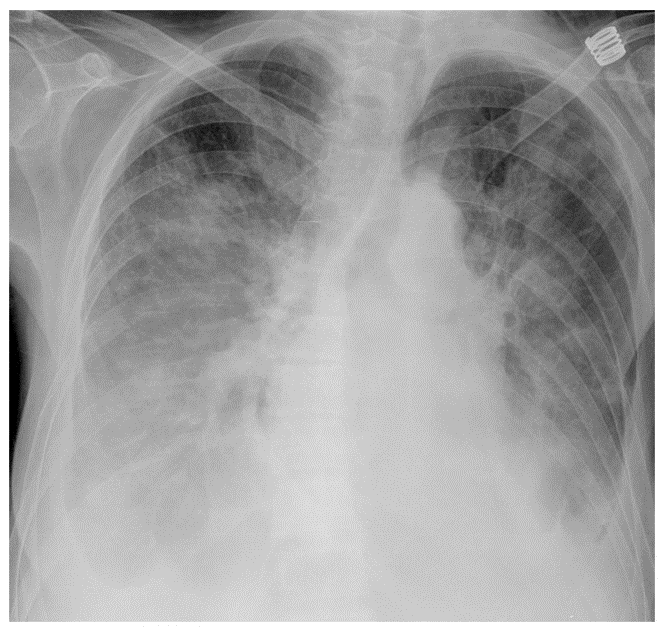
\includegraphics[width=0.3\textwidth]{./imagenes/UCIDoc-SVICasoARXTorax.png}
      \caption{\label{fig:Brusilov:SVI:CasoARXTorax}Placa de rayos X del tórax complementaria.}
    \end{subfigure}
    \caption{\label{fig:Brusilov:SVI:PruebasCasoB}Pruebas complementarias del Caso B.}
\end{figure}

\begin{figure}[hptb]
    \centering
	\includegraphics[width=0.766\linewidth]{./imagenes/ACV-AdSC-CasosUCI_CasoB.png}
	\caption{\label{fig:Brusilov:SVI:CasoB}Flujograma y resolución del Caso B.}
\end{figure}
\clearpage

\subsection{Caso C - Neumotórax a tensión}
\paragraph{Escenario} UCI
\vspace{-12.5pt}
\paragraph{Paciente} Varón de 60 años ingresa en la UCI por una sepsis urinaria. Allí se le coloca una vía central subclavia derecha y un catéter arterial radial y se le aplica tratamiento con noradrenalina y antibióticos. En el momento de la exploración, presenta hipotensión (70/40 mm Hg), taquicardia (150 lpm), taquiapnea (35 rpm) y saturación de O$_2$ de 83 \%. Ante la auscultación pulmonar, presenta abolición del murmullo vesicular en el hemitórax derecho.
\vspace{-12.5pt}
\paragraph{Caso} Se avisa al personal médico de guardia. El paciente algo confuso relata la historia clínica y que . A los 80 segundos, el paciente presenta una bradicardia sinusal brusca y al llegar a 30 lpm (20 seg), entra en asistolia. Se espera que el alumnado realice el protocolo de RCP no desfibrilable:
\begin{enumerate}[topsep=0pt, partopsep=0pt,itemsep=0pt,parsep=0pt]
    \item Colocación de tablero de RCP.
    \item Inicio de compresiones y asistencia de vía aérea con Ambú (30:2).
    \item Canalización de vía venosa, junto con administración de medicación (adrenalina cada 3 minutos).
    \item Si el alumnado no progresa (sólo hace compresiones), recordar las posibles causas de parada (<<4H y 4T>>). El paciente solo saldrá si se realiza una descompresión mediante aguja en el segundo espacio intercostal.
\end{enumerate}
\vspace{-12.5pt}
\paragraph{Pruebas complementarias}
\begin{itemize}[topsep=0pt, partopsep=0pt,itemsep=0pt,parsep=0pt]
    \item \textbf{Gasometría post-parada}: pH 7,20; pCO$_2$ 70; pO$_2$ 20; EB -10; lact 6; Hb 15; HCO$_3^-$ 18; K$^+$ 4.
    \item \textbf{Electrocardiograma previo}: \href{https://drive.google.com/file/d/192ypfJwq66tplKSGUsnxHWUPYwEQuJeX/view?usp=share\_link}{Enlace Drive ECG}
    \item \textbf{Placa rayos X torácica}: \href{https://drive.google.com/file/d/1_oLDL2m2RXA4fkvJ76m1YXThYZ4J_dJR/view?usp=share\_link}{Enlace Drive RX tórax}
\end{itemize}
\begin{figure}[hptb]
    \centering
    \begin{subfigure}{.5\textwidth}
      \centering
      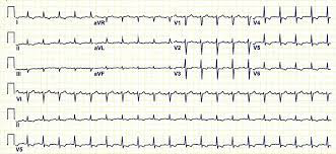
\includegraphics[width=0.7\textwidth]{./imagenes/UCIDoc-SVICasoCECG.png}
      \caption{\label{fig:Brusilov:SVI:CasoCECG}Electrocardiograma complementario.}
    \end{subfigure}%
    \begin{subfigure}{.5\textwidth}
      \centering
      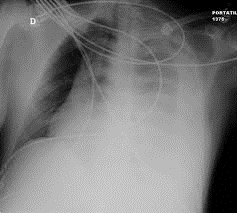
\includegraphics[width=0.4\textwidth]{./imagenes/UCIDoc-SVICasoCRXTorax.png}
      \caption{\label{fig:Brusilov:SVI:CasoCRXTorax}Placa de rayos X del tórax complementaria.}
    \end{subfigure}
    \caption{\label{fig:Brusilov:SVI:PruebasCasoC}Pruebas complementarias del Caso C.}
\end{figure}

\begin{figure}[hptb]
    \centering
	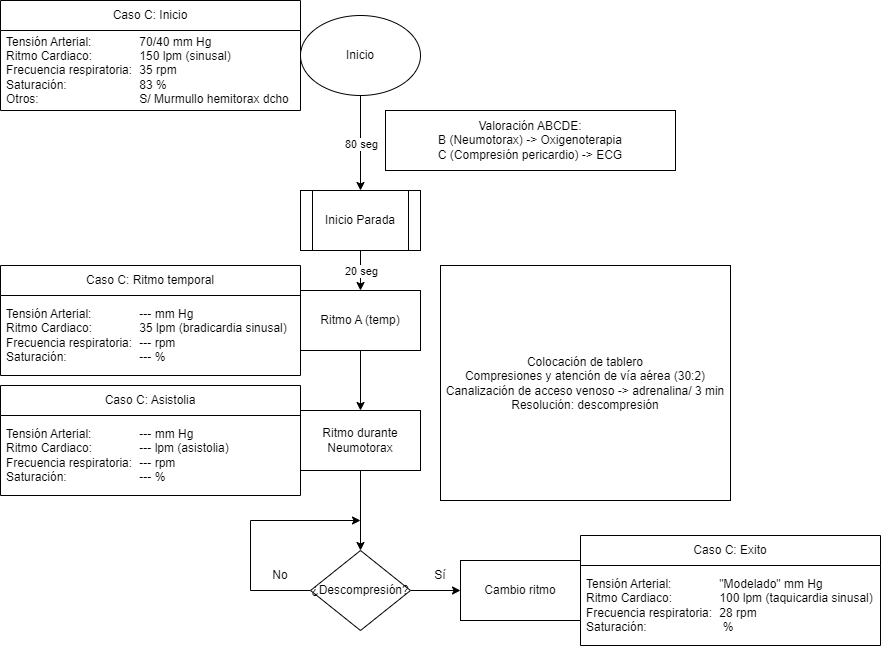
\includegraphics[width=0.8\linewidth]{./imagenes/ACV-AdSC-CasosUCI_CasoC.png}
	\caption{\label{fig:Brusilov:SVI:CasoC}Flujograma y resolución del Caso C.}
\end{figure}
\clearpage


